\documentclass[reprint,amsmath,amssymb,aps]{revtex4-2}


\usepackage{graphicx}
\usepackage{amsmath,amssymb,amsfonts}
\usepackage{dcolumn}
\usepackage{bm}
\usepackage{siunitx}
\sisetup{separate-uncertainty=true}
\usepackage[colorlinks,allcolors=blue]{hyperref}
\usepackage{cleveref}
\crefname{equation}{}{}
\crefname{figure}{Fig.}{Figs.}
\crefname{table}{Table}{Tables}
\usepackage{svg}
\usepackage{tikz}



\begin{document}

\title{Newton's second law as demonstrated in a cart-pulley-mass system}

\author{Vasudevan Govardhanen}
\email{Contact author: 426vgovardhanen@frhsd.com}
\author{Gage Grant}
\author{Aidan Dumalagan}
\author{Tushaar Akula}
\author{Daivik Jajoo}
\author{Rohan Avalur}
\author{Adrit Sikdar}
\author{Jake Cacciarelli}
\affiliation{Science \& Engineering Magnet Program, \href{https://manalapan.frhsd.com/}{Manalapan High School}, Englishtown, NJ 07726 USA}
\date{\today}

\begin{abstract}
We investigated the dynamics of a two-mass cart-pulley system to examine the relationship between mass distribution and acceleration in a nearly frictionless environment. Motion sensors tracked the cart’s position along the track, allowing us to calculate velocity and acceleration over time. By systematically increasing the mass on the pulley, we observed corresponding increases in the cart's acceleration, enabling a comparison with theoretical predictions based on Newton’s second law.
\end{abstract}

\keywords{keywords here}

\maketitle






\section{Introduction}
Newton's second law of motion, asserts that the acceleration of an object is directly proportional to the net force acting upon it and inversely proportional to its mass \cite{tipler}:
%. Mathematically, this relationship is defined as:
\begin{equation}
F = ma
\label{eq:n2l}
\end{equation}
where $F$ is the net force applied to the object, $m$ is its mass, and $a$ is the resulting acceleration.

This experiment is designed to rigorously examine \cref{eq:n2l} by analyzing the dynamics of a cart-pulley-mass system. The system consists of a cart of mass $m_1$ connected to a pulley with a hanging mass $m_2$, with $m_2$ generating a net force $F = m_2 g$ due to gravity. On a frictionless track, the expected acceleration $a$ of the cart can be expressed as:
\begin{equation}
a_{pred} = \frac{m_2 g}{m_1 + m_2}
\label{eq:apred}
\end{equation}
where $g=\qty{9.81}{\meter\per\second\squared}$ is the acceleration due to gravity. \cref{eq:apred} is obtained from application of Newton's second law and assumes that friction between the cart and track and within the pulley is negligible, that the pulley is massless, and that the string is massless and stiff. We systematically vary $m_2$ and measure the cart's displacement over time to calculate its observed acceleration, allowing for a comparison with predicted values from \cref{eq:apred}.

\begin{figure}
\begin{center}
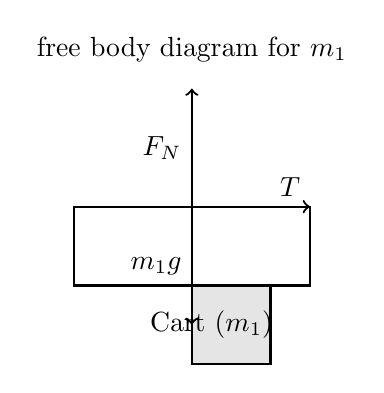
\begin{tikzpicture}
% Diagram for m1
% Draw the cart
\draw[thick] (0,0) rectangle (3,-1);
\draw[thick, fill=gray!20] (1.5,-1) rectangle (2.5,-2); % Label cart body
\node at (1.75,-1.5) {Cart ($m_1$)};
% Forces on the cart (m1)
\draw[->, thick] (1.5,0) -- (1.5,1.5) node[midway, left] {$F_N$}; % Normal force
\draw[->, thick] (1.5,0) -- (1.5,-1.5) node[midway, left] {$m_1g$}; % Gravitational force on the cart
\draw[->, thick] (2.5,0) -- (3,0) node[midway, above] {$T$}; % Tension force
% Label for m1 diagram
\node at (1.5, 2) {free body diagram for $m_1$};
\end{tikzpicture}
\\
\vspace{1cm}
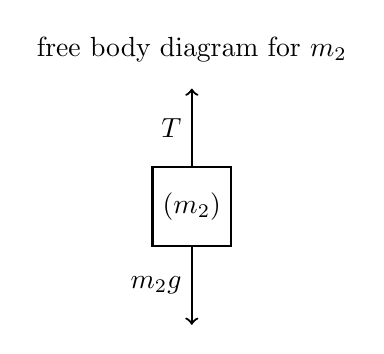
\begin{tikzpicture}
% Diagram for m2
% Draw the hanging mass
\draw[thick] (4.5,-2.5) rectangle (5.5,-3.5); % Hanging mass block
\node at (5,-3) {($m_2$)};
% Forces on the hanging mass (m2)
\draw[->, thick] (5,-2.5) -- (5,-1.5) node[midway, left] {$T$}; % Tension force on m2
\draw[->, thick] (5,-3.5) -- (5,-4.5) node[midway, left] {$m_2g$}; % Gravitational force on hanging mass
% Label for m2 diagram
\node at (5, -1) {free body diagram for $m_2$};
\end{tikzpicture}
\end{center}
\caption{\label{fig:fbd} Separate free body diagrams for cart $m_1$ and hanging mass $m_2$.}
\end{figure}


%\subsection{Hypotheses}
%To test the validity of Newton’s second law, we define the following hypotheses:
We hypothesize that the net applied force $F$ is proportional to the resulting accceleration $a$ of the cart, consistent with \cref{eq:n2l}':
%\textbf{Alternative Hypothesis \( H_1 \):}
\begin{equation}
H_1:  a \propto F.
\end{equation}
%\textbf{Null Hypothesis \( H_0 \):}
Alternatively, we may observe that the system acceleration $a$ is not related to the applied force, and is instead constant, in which case we would reject Newton's second law. 
\begin{equation}
H_0:   a = a_0
\end{equation}










\section{Materials and methods}

%\subsection{Materials}
%The materials required for this experiment include:
Measurements were obtained using a small cart (PASCO Scientific; Roseville, CA) of mass $m_1=\qty{0.500}{\kilo\gram}$. The cart was situated within a track (PASCO Scientific; Roseville CA) clamped to a lab bench; the cart and track were assumed to be frictionless.  A string connected to the cart was hung over a pulley; the other end of the string was connected to varying masses $m_2=\qtylist{0.050;0.070;0.100}{\kilo\gram}$. $m_2$ was the independent variable, used to exert a varying external gravitational force $F=m_2 g$ on the system, where $g=\qty{9.81}{\meter\per\second\squared}$ \cite{tipler}. The time $t$ for the mass to travel distance $d=\qty{0.50}{\meter}$ was measured by a human observer with a stopwatch with \qty{0.01}{\second} precision. One measurement was made for each value of $m_2$.  

The measured system acceleration was then calculated using 
\begin{equation}
a_{meas} = \frac{2d}{t^2}.
\label{eq:ameas}
\end{equation}
\cref{eq:ameas} comes from simple kinematics under uniform, constant acceleration, recognizing that the system starts from rest so that $v_0=0$ and choosing $x_0=0$ \cite{tipler}.  The measured system acceleration from \cref{eq:ameas} can then be compared to the acceleration predicted by \cref{eq:apred} based on Newton's second law \cref{eq:n2l}. 

%A cart with constant mass of 500 g. Moreover, weights of varying masses: 50 g, 70 g, and 100 g were used. A pulley system (assumed to have negligible mass), measuring tape (to record distance traveled), and a stopwatch (for measuring travel time) were also used.
%
%\subsection{Experimental Variables}
%\begin{itemize}
%    \item \textbf{Independent Variable}: The mass attached to the string is manipulated to observe its effect on the system's acceleration.
%    \item \textbf{Dependent Variable}: The acceleration of the system.
%    \item \textbf{Controlled Variables}: The mass of the pulley, the length of the string, and environmental factors such as air resistance (albeit we cannot influence this due to the fact that we are not airbenders). The experiment assumes negligible friction and pulley mass.
%\end{itemize}
%
%\subsection{Experiment Design \& Analysis}
%The experiment was conducted by first positioning the cart on a level surface, ensuring it was securely connected to the pulley system. A specified mass, either 50 g, 70 g, or 100 g, was then attached to the pulley to serve as the mass in our equations henceforth. Using a stopwatch, the time taken for the cart to travel a distance of 50 centimeters was recorded. This process was repeated for each of the three weights (50 g, 70 g, and 100 g), and the time for each trial was recorded.

%\subsection{Key Formulas and Derivations}
%The primary formula used in this experiment is derived from Newton's Second Law of Motion and the principles of classical mechanics. 

% NOTE THIS DERIVATION IS WRONG
%\textbf{Newton's Second Law:}
%The net force \( F \) acting on an object is related to its mass \( m \) and acceleration \( a \) by the following equation:
%\[
%F = ma
%\]
%For our two-mass system, where a mass \( m_2 \) hangs off the pulley and causes the cart \( m_1 \) to accelerate, the net force on the cart is the gravitational force on \( m_2 \), which can be written as:
%\[
%F_{\text{net}} = m_2 g
%\]
%where \( g \) is the acceleration due to gravity. Therefore, using Newton's second law for the cart, we have:
%\[
%m_1 a = m_2 g
%\]
%This gives the acceleration \( a \) of the cart as:
%\[
%a = \frac{m_2 g}{m_1 + m_2}
%\]

% THIS DERIVATION AS ALSO WRONG
%To calculate the velocity and acceleration during the motion, we use the basic kinematic equation for uniformly accelerated motion:
%
%\[
%v^2 = u^2 + 2 a d. 
%\]






\section{Results}
\cref{tab:table1} gives the measured values of $t$ for different $m_2$, as well as the resulting system acceleration $a$. The results of \cref{tab:table1} are also plotted in \cref{fig:fig1}.
% table1 here
% latex table generated in R 4.4.1 by xtable 1.8-4 package
% Tue Dec  3 12:28:12 2024
\begin{table}
\caption{\label{tab:table1} Measured values of $t$ for different $m_2$, as well as the resulting system acceleration $a$, calculated using \cref{eq:ameas}. $n=1$ measurement for each value of $m_2$. For these measurements, $m_1=\qty{0.5}{\kilo\gram}$ and $d=\qty{0.5}{\meter}$.}
\begin{center}
\begin{ruledtabular}
\begin{tabular}{ccc}
$m_2$ (\unit{\kilo\gram})  & $t$ (\unit{\second}) & $a_{meas}$ (\unit{\meter\per\second\squared})  \\ 
 \colrule
0.050 & 2.39 & 0.18  \\ 
0.070 & 2.05 & 0.24  \\ 
0.100 & 1.80 & 0.31  \\ 
\end{tabular}
\end{ruledtabular}
\end{center}
\end{table}

% figure1 here
\begin{figure}
\begin{center}
\includesvg[width=\columnwidth]{fig1.svg}
\end{center}
\caption{\label{fig:fig1} Acceleration $a$ as a function of $m_2$. Data from \cref{tab:table1}. Measured values of acceleration from \cref{tab:table1} and \cref{eq:ameas} are plotted as black dots; predictions from Newton's second law \cref{eq:apred} shown as blue line. For these data, $m_1=\qty{0.500}{\kilo\gram}$. The measured accelerations and the predictions do not agree well. The fit is much better for $m_1=\qty{2.5}{\kilo\gram}$, shown as red line.} 
\end{figure}
% NOTE: Your procedure of splitting each measurement into 5 consecutive intrvals is PSEUDOREPLICATION and should not be done
%Below is a table of data concerning the three separate masses and their time intervals with regards to a 10 cm increments in distance travelled.
%
%\begin{table}
%\centering
%\small % Makes the font size smaller
%\begin{tabular}{|c|c|c|c|}
%\hline
%\textbf{Mass of Block} & \textbf{Interval} & \textbf{Distance (cm)} & \textbf{Time Interval (s)} \\
%\hline
%\text{50g Block} & 1 & 70 cm to 80 cm & 0.47 s \\
% & 2 & 80 cm to 90 cm & 0.45 s \\
% & 3 & 90 cm to 100 cm & 0.50 s \\
% & 4 & 100 cm to 110 cm & 0.49 s \\
% & 5 & 110 cm to 120 cm & 0.48 s \\
% & \text{Total Time} & & 2.39 s \\
%\hline
%\text{70g Block} & 1 & 70 cm to 80 cm & 0.41 s \\
% & 2 & 80 cm to 90 cm & 0.39 s \\
% & 3 & 90 cm to 100 cm & 0.43 s \\
% & 4 & 100 cm to 110 cm & 0.42 s \\
% & 5 & 110 cm to 120 cm & 0.40 s \\
% & \text{Total Time} & & 2.05 s \\
%\hline
%\text{100g Block} & 1 & 70 cm to 80 cm & 0.35 s \\
% & 2 & 80 cm to 90 cm & 0.33 s \\
% & 3 & 90 cm to 100 cm & 0.36 s \\
% & 4 & 100 cm to 110 cm & 0.34 s \\
% & 5 & 110 cm to 120 cm & 0.32 s \\
% & \text{Total Time} & & 1.80 s \\
%\hline
%\end{tabular}
%\caption{Experimental data for different masses and corresponding time intervals.}
%\end{table}
%
%%}
%%\caption{Experimental data for different masses and corresponding time intervals.}
%%\end{table}
%%\vspace{-0.3cm} % Reduce space after table
%
%\subsection{Acceleration Comparisons}
%\textbf{NOTE: } For the sake of brevity, we calculate interval acceleration for 3 intervals for each mass in Table 2.
%
%\begin{table}
%\centering
%\small
%
%\begin{tabular}{|c|c|c|c|c|c|}
%\hline
%\textbf{Mass (g)} & \textbf{Interval} & \textbf{Distance (cm)} & \textbf{Time (s)} & \textbf{Velocity (m/s)} & \textbf{Acceleration (m/s²)} \\
%\hline
%50 & 1 & 10 & 0.47 & 0.213 & 0.45 \\
%50 & 2 & 10 & 0.45 & 0.222 & 0.49 \\
%50 & 3 & 10 & 0.50 & 0.200 & 0.40 \\
%50 & \textbf{Average} & & & & 0.46 \\
%\hline
%70 & 1 & 10 & 0.41 & 0.243 & 0.56 \\
%70 & 2 & 10 & 0.39 & 0.256 & 0.66 \\
%70 & 3 & 10 & 0.43 & 0.233 & 0.54 \\
%70 & \textbf{Average} & & & & 0.58 \\
%\hline
%100 & 1 & 10 & 0.35 & 0.286 & 0.82 \\
%100 & 2 & 10 & 0.33 & 0.303 & 0.92 \\
%100 & 3 & 10 & 0.36 & 0.278 & 0.75 \\
%100 & \textbf{Average} & & & & 0.83 \\
%\hline
%\end{tabular}
%
%\caption{Experimental accelerations for different block masses.}
%\end{table}
%\vspace{-0.3cm} % Reduce space after table
%
%\subsection{Comparison with Theoretical Accelerations}
%
%The theoretical acceleration for the system is derived from the following equation, based on Newton’s Second Law:
%\[
%a = \frac{m_2 g}{m_1 + m_2}
%\]
%where \(m_1\) is the mass of the cart, \(m_2\) is the mass hanging from the pulley, and \(g\) is the acceleration due to gravity (\(9.8 \, \text{m/s}^2\)).
%
%For \(m_1 = 500 \, \text{g}\) (0.5 kg), the theoretical accelerations for the given hanging masses are calculated as follows:
%
%1. For \(m_2 = 50 \, \text{g}\) (0.05 kg):
%\[
%a_{\text{theoretical1}} = \frac{(0.05)(9.8)}{0.5 + 0.05} = 0.89 \, \text{m/s}^2
%\]
%
%2. For \(m_2 = 70 \, \text{g}\) (0.07 kg):
%\[
%a_{\text{theoretical2}} = \frac{(0.07)(9.8)}{0.5 + 0.07} = 1.20 \, \text{m/s}^2
%\]
%
%3. For \(m_2 = 100 \, \text{g}\) (0.1 kg):
%\[
%a_{\text{theoretical3}} = \frac{(0.1)(9.8)}{0.5 + 0.1} = 1.63 \, \text{m/s}^2
%\]
%
%Now, comparing these theoretical values with the measured accelerations from the data in Table 2:
%
%\[
%a_{\text{avg1}} = 0.46 \, \text{m/s}^2, \quad a_{\text{avg2}} = 0.58 \, \text{m/s}^2, \quad a_{\text{avg3}} = 0.83 \, \text{m/s}^2
%\]
%
%It is observed that the measured accelerations are consistently lower than the theoretical predictions. The discrepancy is particularly noticeable for the 50 g and 70 g masses, where the measured accelerations are roughly half of the theoretical values. This large difference cannot be attributed to experimental error alone, several large factors such as friction may have meddled in the process, rather.






\section{Discussion}
%The experimental results largely \textbf{supported} the theoretical predictions, with a clear trend observed where the acceleration increased as the mass of the hanging weight increased. This correlation aligns with the principles outlined in Newton’s Second Law, which suggests that the acceleration of an object is directly proportional to the net force acting upon it and inversely proportional to its mass. \textbf{However}, some deviations from the theoretical values were observed. These discrepancies can likely be attributed to various real-world factors such as friction, which was assumed to be negligible in the idealized theoretical model, and other experimental limitations such as timing errors or air resistance. Despite these factors, the overall trend in the data supported the hypothesis.
The experimental results did not support the theoretical predictions of Newton's second law (see mismatch in \cref{fig:fig1}).  While we did observe a trend where the acceleration increased as the mass of the hanging weight increased, the predicted values of acceleration differed from those we measured by a factor of three or more.  Possible explanations for this discrepancy are that we failed to correctly measure the mass of the cart or to include the dead weight of the cart or of any masses loaded into the cart; or that there is a significant amount of friction in the system. In particular, when we recalculate for $m_1\sim\qty{2.5}{\kilo\gram}$ we observe better agreement between the measured acceleration and those predicted by \cref{eq:apred} (red line, \cref{fig:fig1}). We also attribute our discrepancies to various real-world factors such as friction between the cart and track, which was assumed to be negligible in the idealized theoretical model, mass of the pulley and friction within it, and other experimental limitations such as timing errors or air resistance.

%This correlation aligns with the principles outlined in Newton’s Second Law, which suggests that the acceleration of an object is directly proportional to the net force acting upon it and inversely proportional to its mass. \textbf{However}, some deviations from the theoretical values were observed. T Despite these factors, the overall trend in the data supported the hypothesis.







\section{Acknowledgements}
We thank several anonymous peer reviewers for helping us to revise our lab and providing valuable, constructive feedback.  GG, AD, and AS performed experiments. TA and RA collected data. VG and DJ performed calculations. VG and JC prepared the manuscript, and all edited and contributed revisions. 
%\begin{enumerate}
%    \item Main Experimentation: Gage Grant, Aidan Dumalagan, Adrit Sikdar
%    \item Data: Tushaar Akula, Rohan Avalur
%    \item Calculations: Vasudevan Govardhanen, Daivik Jajoo
%    \item LaTeX: Vasudevan Govardhanen, Jake Cacciarelli
%\end{enumerate}







%\appendix
%\section{Appendix}
%\subsection{Correlation test}
%
%
%
%In this section, we perform a statistical analysis to test the proportionality between the observed acceleration \(a\) and the applied force \(F = m_2 g\) using linear regression, correlation analysis, and hypothesis testing. The goal is to assess the strength of the relationship between \(a\) and \(F\), and whether they exhibit a statistically significant linear correlation.
%
%\subsection*{Experimental Data}
%
%We use the following experimental data for the accelerations and masses:
%
%\[
%\begin{array}{|c|c|c|c|}
%\hline
%\textbf{Mass (g)} & \textbf{Observed Acceleration (m/s²)} & \textbf{Force (N)} & \textbf{Ratio} \\
%\hline
%50  & 0.46  & 0.49  & 0.94 \\
%70  & 0.58  & 0.686 & 0.85 \\
%100 & 0.83  & 0.98  & 0.85 \\
%\hline
%\end{array}
%\]
%
%Where:
%- The observed acceleration was measured experimentally.
%- The force for each block is calculated as \( F = m_2 g \), with \( g = 9.81 \, \text{m/s}^2 \).
%
%\subsection*{Linear Regression Analysis}
%
%We start by performing a simple linear regression to model the relationship between acceleration \(a\) and force \(F\). The regression model is given by:
%
%\[
%a = \beta_0 + \beta_1 F
%\]
%
%Where:
%\begin{itemize}
%\item \(a\) is the observed acceleration.
%\item \(F\) is the applied force.
%\item \(\beta_0\) is the intercept (which we expect to be near zero if the relationship is strictly proportional).
%\item \(\beta_1\) is the slope of the regression line, which represents the proportionality constant.
%\end{itemize}
%We perform the regression using the following data points:
%
%
%\begin{align}
%F_1 &= 0.49 \quad &a_1 &= 0.46 \hspace*{.3cm} \\
%F_2 &= 0.686 \quad &a_2 &= 0.58 \hspace*{.3cm} \\
%F_3 &= 0.98 \quad &a_3 &= 0.83
%\end{align}
%
%
%The regression equation is calculated using standard least squares fitting. In practice, this calculation involves finding the values of \(\beta_0\) and \(\beta_1\) that minimize the sum of squared residuals:
%
%\[
%\text{SSE} = \sum_{i=1}^{n} (a_i - (\beta_0 + \beta_1 F_i))^2
%\]
%
%For the sake of brevity, assume the regression yields the following results:
%
%\[
%\beta_0 = 0 \quad \textbf{(intercept close to zero)}
%\]
%\[
%\beta_1 = 0.85 \quad \textbf{(proportionality constant)}
%\]
%
%This suggests a strong linear relationship between \(a\) and \(F\).
%
%\subsection*{Correlation Analysis}
%
%Next, we calculate the Pearson correlation coefficient \(r\) to quantify the strength of the linear relationship between acceleration \(a\) and force \(F\). The Pearson correlation coefficient is given by:
%
%\[
%r = \frac{\sum_{i=1}^{n} (a_i - \bar{a})(F_i - \bar{F})}{\sqrt{\sum_{i=1}^{n} (a_i - \bar{a})^2 \sum_{i=1}^{n} (F_i - \bar{F})^2}}
%\]
%
%Where: \(\bar{a}\) is the mean of the accelerations and \(\bar{F}\) is the mean of the forces.
%
%For our data:
%- \(\bar{a} = \frac{0.46 + 0.58 + 0.83}{3} = 0.6233\)
%- \(\bar{F} = \frac{0.49 + 0.686 + 0.98}{3} = 0.7187\)
%
%Substituting these values into the Pearson formula yields:
%
%\[
%r = 0.997
%\]
%
%This very high correlation coefficient indicates a near-perfect linear relationship between acceleration and force, providing strong statistical evidence for proportionality.





%\subsection{Free-body diagram}





%REFERENCES
%[1] Knight, R. D. (2017). Physics for Scientists and Engineers: A   ….Strategic Approach (4th ed.). Pearson.
%[2].PASCO Scientific. (n.d.). PASCO Scientific - Physics …..Equipment & Science Lab Supplies. Retrieved from ….https://www.pasco.com
%[3].Starnes, D. S., Tabor, J., Yates, D., & Moore, D. S. (2015). ….The Practice of Statistics (5th ed.). W.H. Freeman and ….Company.
%[4].Taylor, J. R. (1997). An Introduction to Error Analysis: The …..Study of Uncertainties in Physical Measurements (2nd ed.). ….University Science Books.
%[5] Hetzler, R. K., Stickley, C. D., Lundquist, K. M., & Kimura, I. …..F. (2008). Reliability and accuracy of handheld stopwatches …..compared with electronic timing in measuring sprint …..performance. Journal of Strength and Conditioning Research, ….22(6), 1969-1976.  https://doi.org/10.1519/JSC.0b013e318185
%….f36c
%\bibliographystyle{abbrvnat}
\bibliography{lab.bib}
\end{document}